En este capítulo se analizan los resultados de la metodología propuesta al fenómeno de robo de vehículos. En la sección \ref{sec:data} se describen la fuente de información utilizada. En la sección \ref{sec:data_processing} los resultados del procesamiento de los datos. Por último, en la sección\ref{sec:quantative}-\ref{sec:qualitative} se realiza un análisis cuantitativo y cualitativo de los resultados.

\section{Datos}
\label{sec:data}

Para este experimento se cuenta con relatos de víctimas del robo de vehículos provistos por la Asociación de Aseguradores de Chile (AACH). Esta base de datos consta con 49015 relatos entre los años 2011-2016, veasé la Figura \ref{img:robberies_aach} para el detalle por año.

\begin{figure}
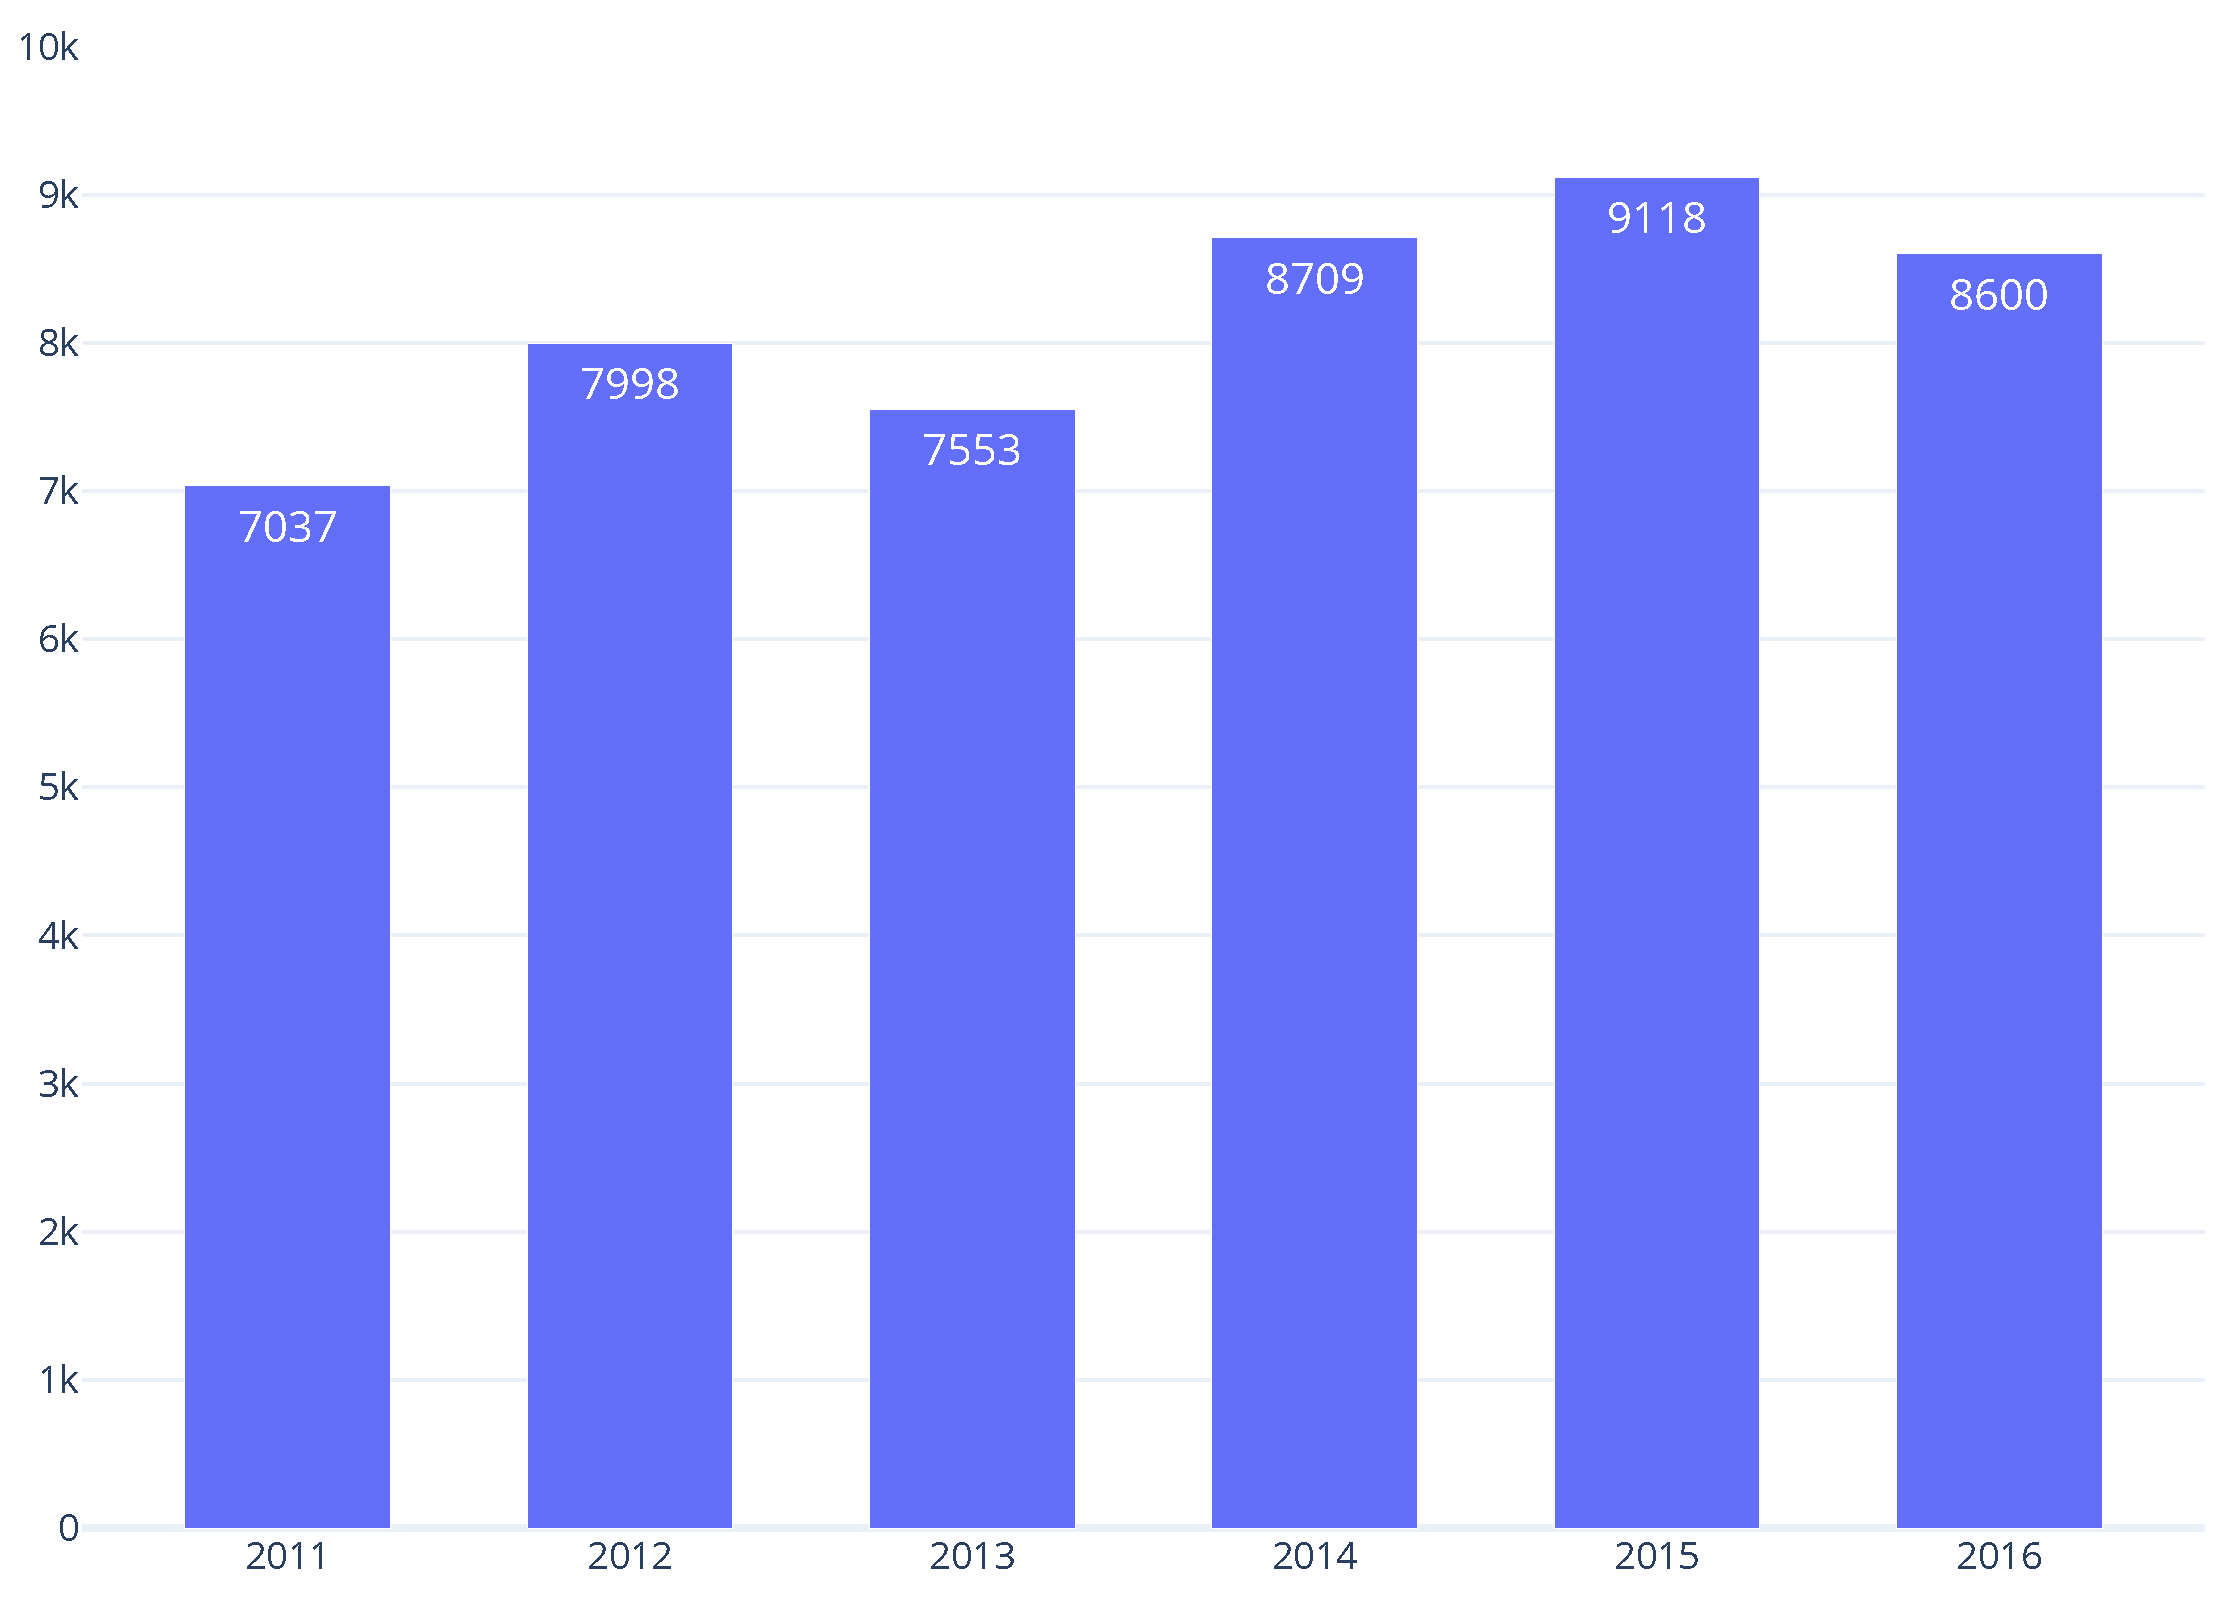
\includegraphics[width=0.8\textwidth]{ch4/robberies_aach.eps}
\caption{Cantidad de robos registrados por año en base de datos AACH.}
\label{img:robberies_aach}
\end{figure}

En la Figura \ref{img:documents} se muestra algunos ejemplos de la base de datos de la AACH, de aquí se observa que los relatos carecen de estandarización y presentan múltiples errores ortográficos. En consecuencia, la etapa de procesamiento toma suma relevancia, ya que aplicar un modelo de tópicos a un corpus sin ningún tipo de procesamiento nos puede llevar a resultados no deseados. En la sección \ref{sec:data_processing} se detallan los resultados obtenidos sobre el corpus tras aplicar los niveles de procesamiento mencionados en la sección \ref{sec:processing}.

\def\grayboxtext[#1,#2]#3{
        \node[fill=gray!80, text width=36em, draw=black!80, rounded corners, align=justify, below=#1] (#2) {#3}; 
}
\begin{figure}
\begin{tikzpicture}
    \grayboxtext[,t1]{\small ESTABA ESTACIONADO EL LA CALLE ROTEMBURGO ENTRE NORUGA Y SEÑORA DEL ROSAIO  Y AL MOMENTO DE IR A BUSCAR EL AUTO SE DA CUENTA QUE EL VH NO SE ENCUETRA AL PARECER LO ROBARON. NO POSEEE LOS DOCUMENTOS DEL VH vh aparece pero con mulples daños e evaluar queda en manos del liquidador.};
    \grayboxtext[0.2cm of t1,t2]{\small ME ENCONTRABA CARGANDO COMBUSTIBLE EN LA SHELL DE CARRASCAL CON WALKER MARTÍNEZ Y REPENTINAMENTE FUI ASALTADA EN FORMA VIOLENTA LLEVASE MI VEH (TENGO GRABACIÓN ). DAÑOS: ROBO DE MI VEH . LEIVA SE DERIVA A DON MARIO MEDINA .3 UF.DED/XX@XX.CL};
    \grayboxtext[0.2cm of t2,t3]{\small TEXT : DEJO MI VEHICULO ESTACIONADO EN DICHO LUGAR AL VOLVER ME PERCATO QUE EL VEHICULO HABIA SIDO ROBADO  EL MISMO DIA DEL ROBO A LAS 20:00 SOY CONTACTADO POR CARABINEROS DE LA COMUNA DE EL BOSQUE LOS CUALES ME INFORMAN QUE HABIAN RECUPERADO MI VEHICULO EL CUAL PRESENTABA LOS SIGUIENTES DAÑOS : VIDRIO TRASERO DERECHO QUEBRADA  CHAPA DE CONTACTO FORZADA  PARACHOQUE DELANTERO DERECHO RAYADO  ALARMADESCONECTADA  OTROS DAÑOS EN EL SISTEMA ELECTRICO  ALARMA DE AIRBAGS ENCENDIDA  ROBO DE ESPECIES.};
    \grayboxtext[0.2cm of t3,t4]{\small Descripción Siniestro: el dia 24 de abril se le arrendo el vh a XX el cual estuvo sin problemas pagando el arriendo  hasta el mes pasado que no pago mas y se le ha llamado en reiteradas veces y dice que va a venir a dejar el auto y no aparecel. por eso se realizo una denuncia por apropiacion indevida};
    \grayboxtext[0.2cm of t4,t5]{\small ammg  53966748    vh asegurado transitaba en calle copiapo alt. 750  en este punto sufro portonazo sujetos armados roban mi vh hoy a las 04.30am vh fue encontrado en sector de la pintana mi vh ahora esta siendo periciado.    daños por evaluar};
    \grayboxtext[0.2cm of t5,t6]{\small PATENTE XX Siendo las 22:30 en la interseccion de san Alfonso con Claudio Gay  un individuo me obliga a bajar del vehiculo apuntandome con una pistola  de inmediato aparecen dos personas mas  las que me suben en la parte trasera del furgon donde constantemente me amenazan con dispararme  me bajan del vehiculo en un potrero cercano a la autopista del sol  teniendome boca abajo golpeandome  luego me colocan un pa?o en la cara perdiendo el conocimiento  al despertar desorientado me dirijo a car};
\end{tikzpicture}
\caption{Muestra de relatos de la base de datos AACH.}
\label{img:documents}
\end{figure}

\section{Procesamiento}
\label{sec:data_processing}

En esta sección se detallan los resultados de aplicar el procesamiento descrito en la sección \ref{sec:processing}. Con fines gráficos los resultados del procesamiento se decriben en un orden distinto al descrito en dicha sección, con el objetivo de mostrar en como estas afectan el tamaño del vocabulario. El orden es el siguiente, (i) tokenización, (ii) procesamiento de caracteres, (iii) eliminación de palabras poco frecuentes, (iv) filtro por vocabulario, (v) eliminación de \textit{stopwords} y (vi) eliminación de documentos con pocas palabras.\\

En la Figura \ref{img:cum_dist1} se muestran la distribución acumulada del corpus original tras solo aplicar tokenización. En este caso los \textit{tokens} totales corresponden a 2030980 asociado a un vocabulario de 93203 palabras.\\

La Figura \ref{img:cum_dist2} muestra los resultados al aplicar la etapa de procesamiento de caracteres, de esta se observa que se reduce el tamaño del vocabulario en cerca de la mitad, específicamente a 42921 palabras, similarmente con la cantidad de \textit{tokens}, que ahora son 1028412.

\begin{figure}
    \centering
    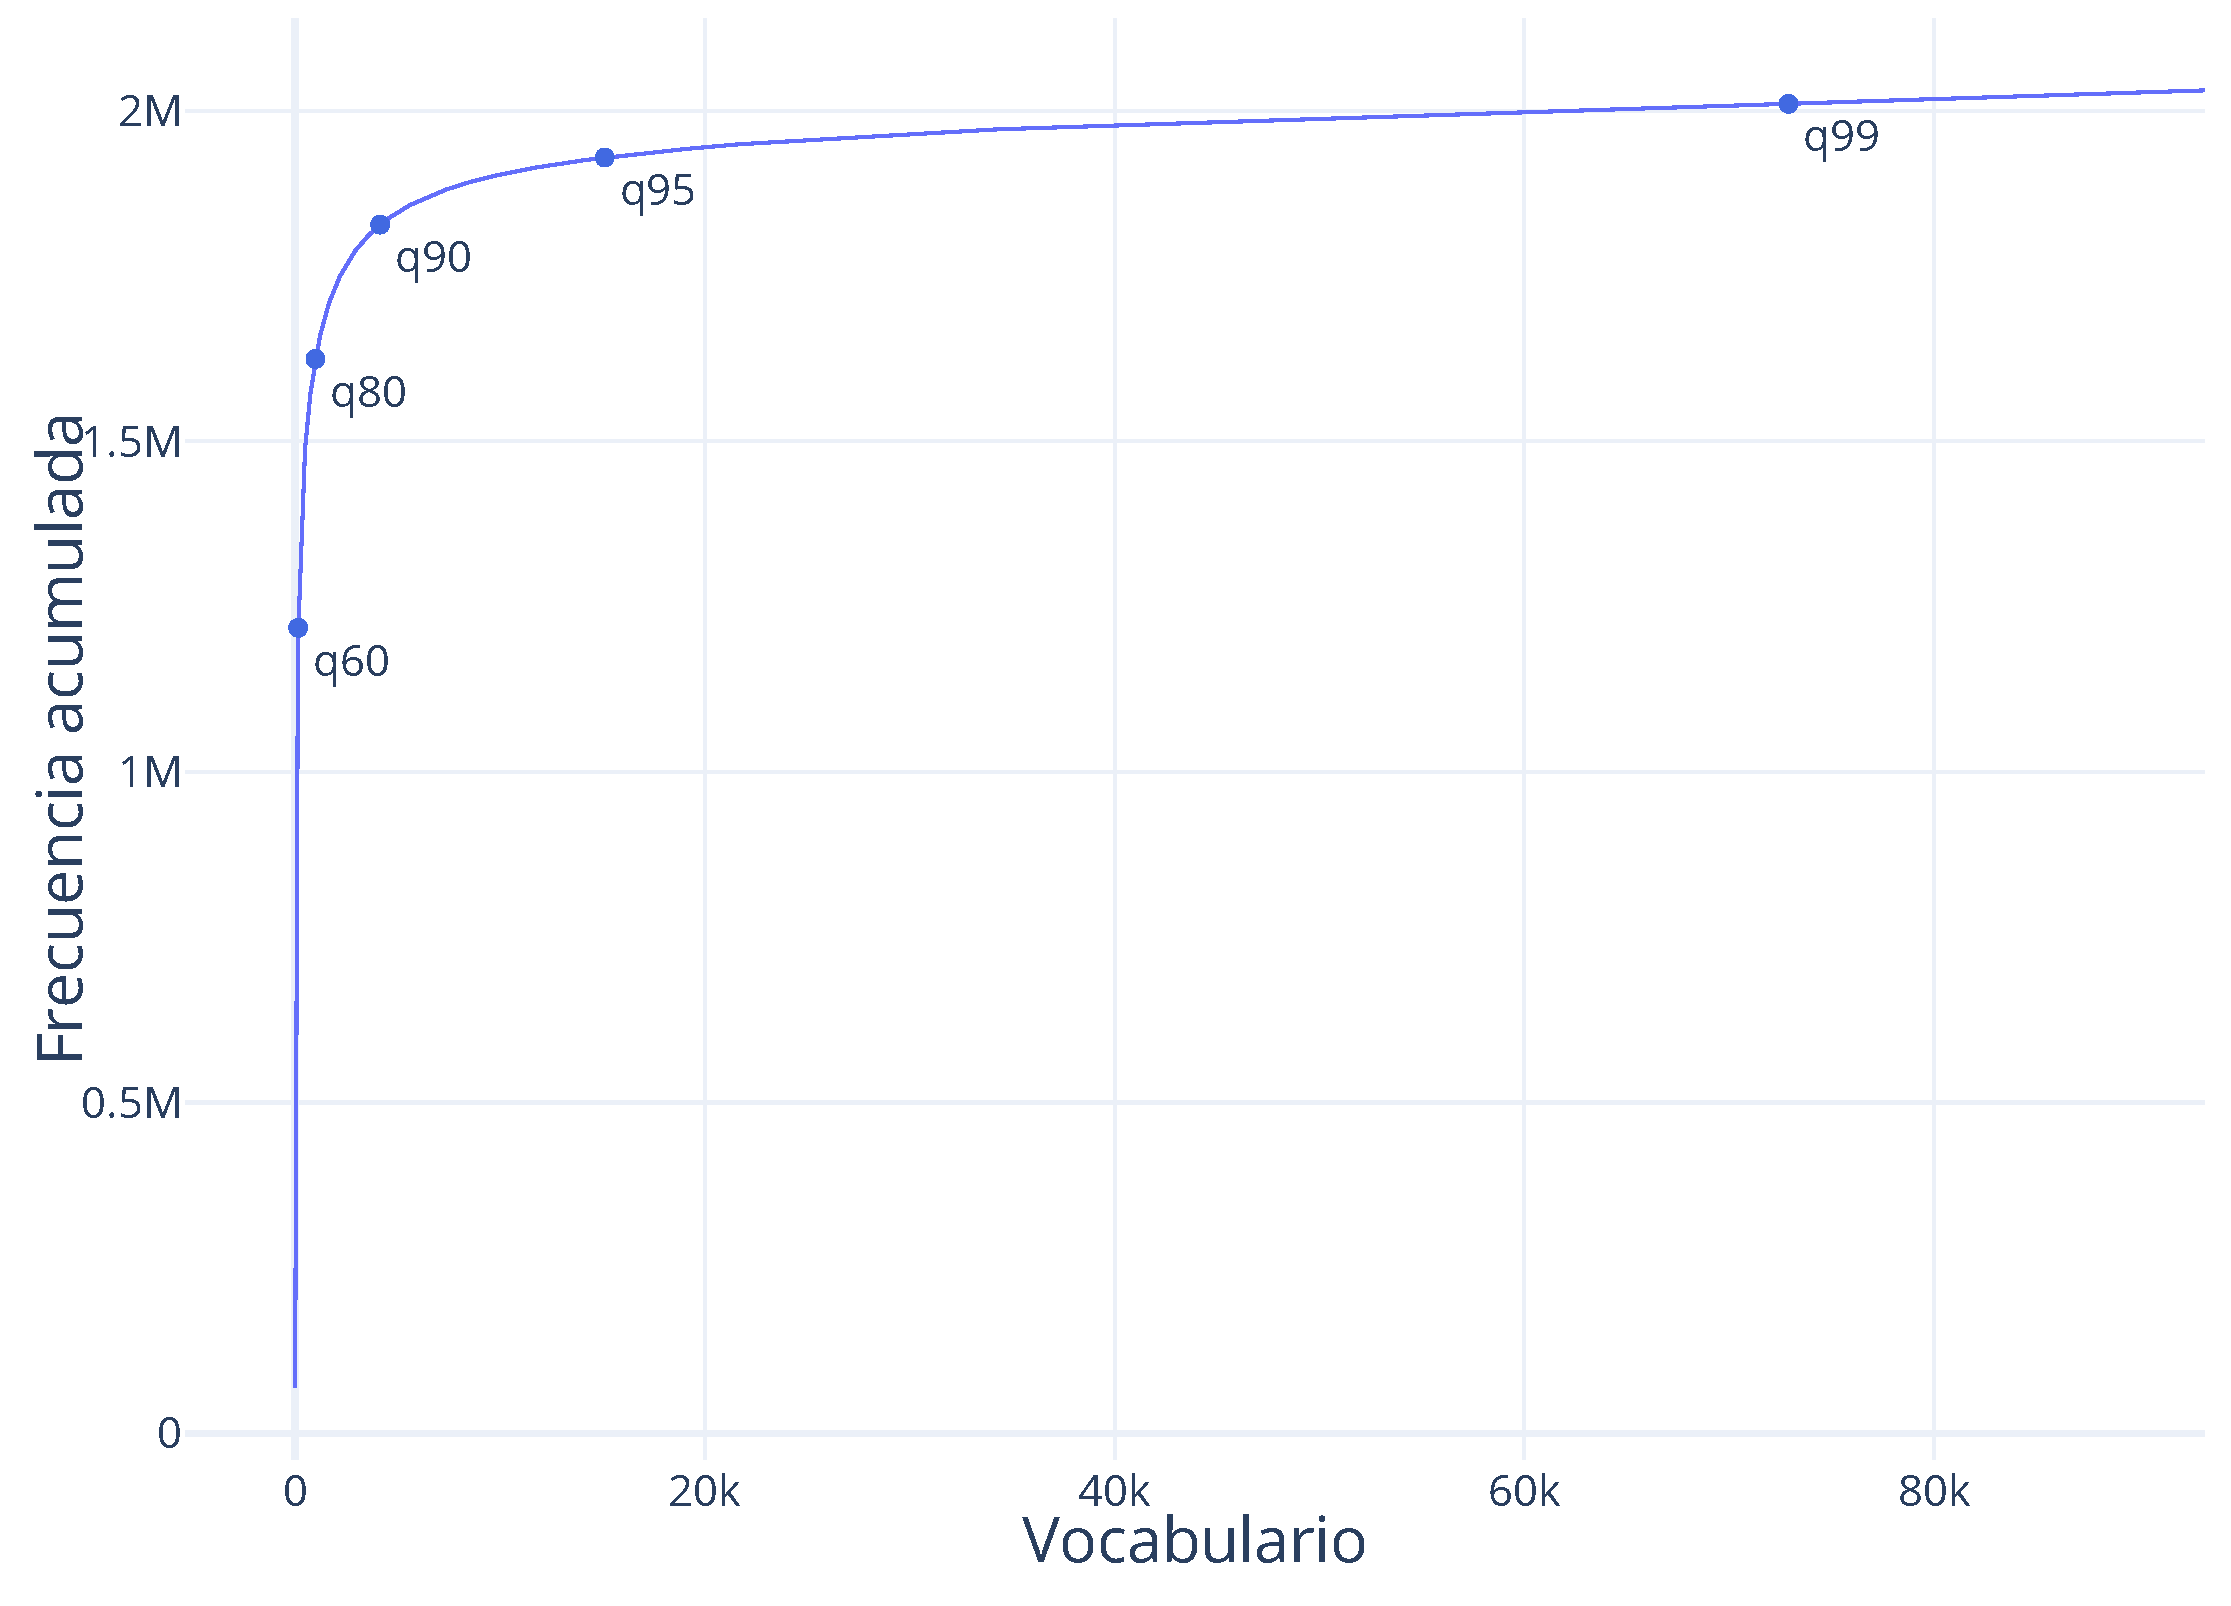
\includegraphics[width=0.8\textwidth]{ch4/cum_dist_1.eps}
    \caption{Frecuencia acumulada del vocabulario en orden decreciente de ocurrencia aplicando hasta el primer nivel de procesamiento.}
    \label{img:cum_dist1}
\end{figure}

\begin{figure}
    \centering
    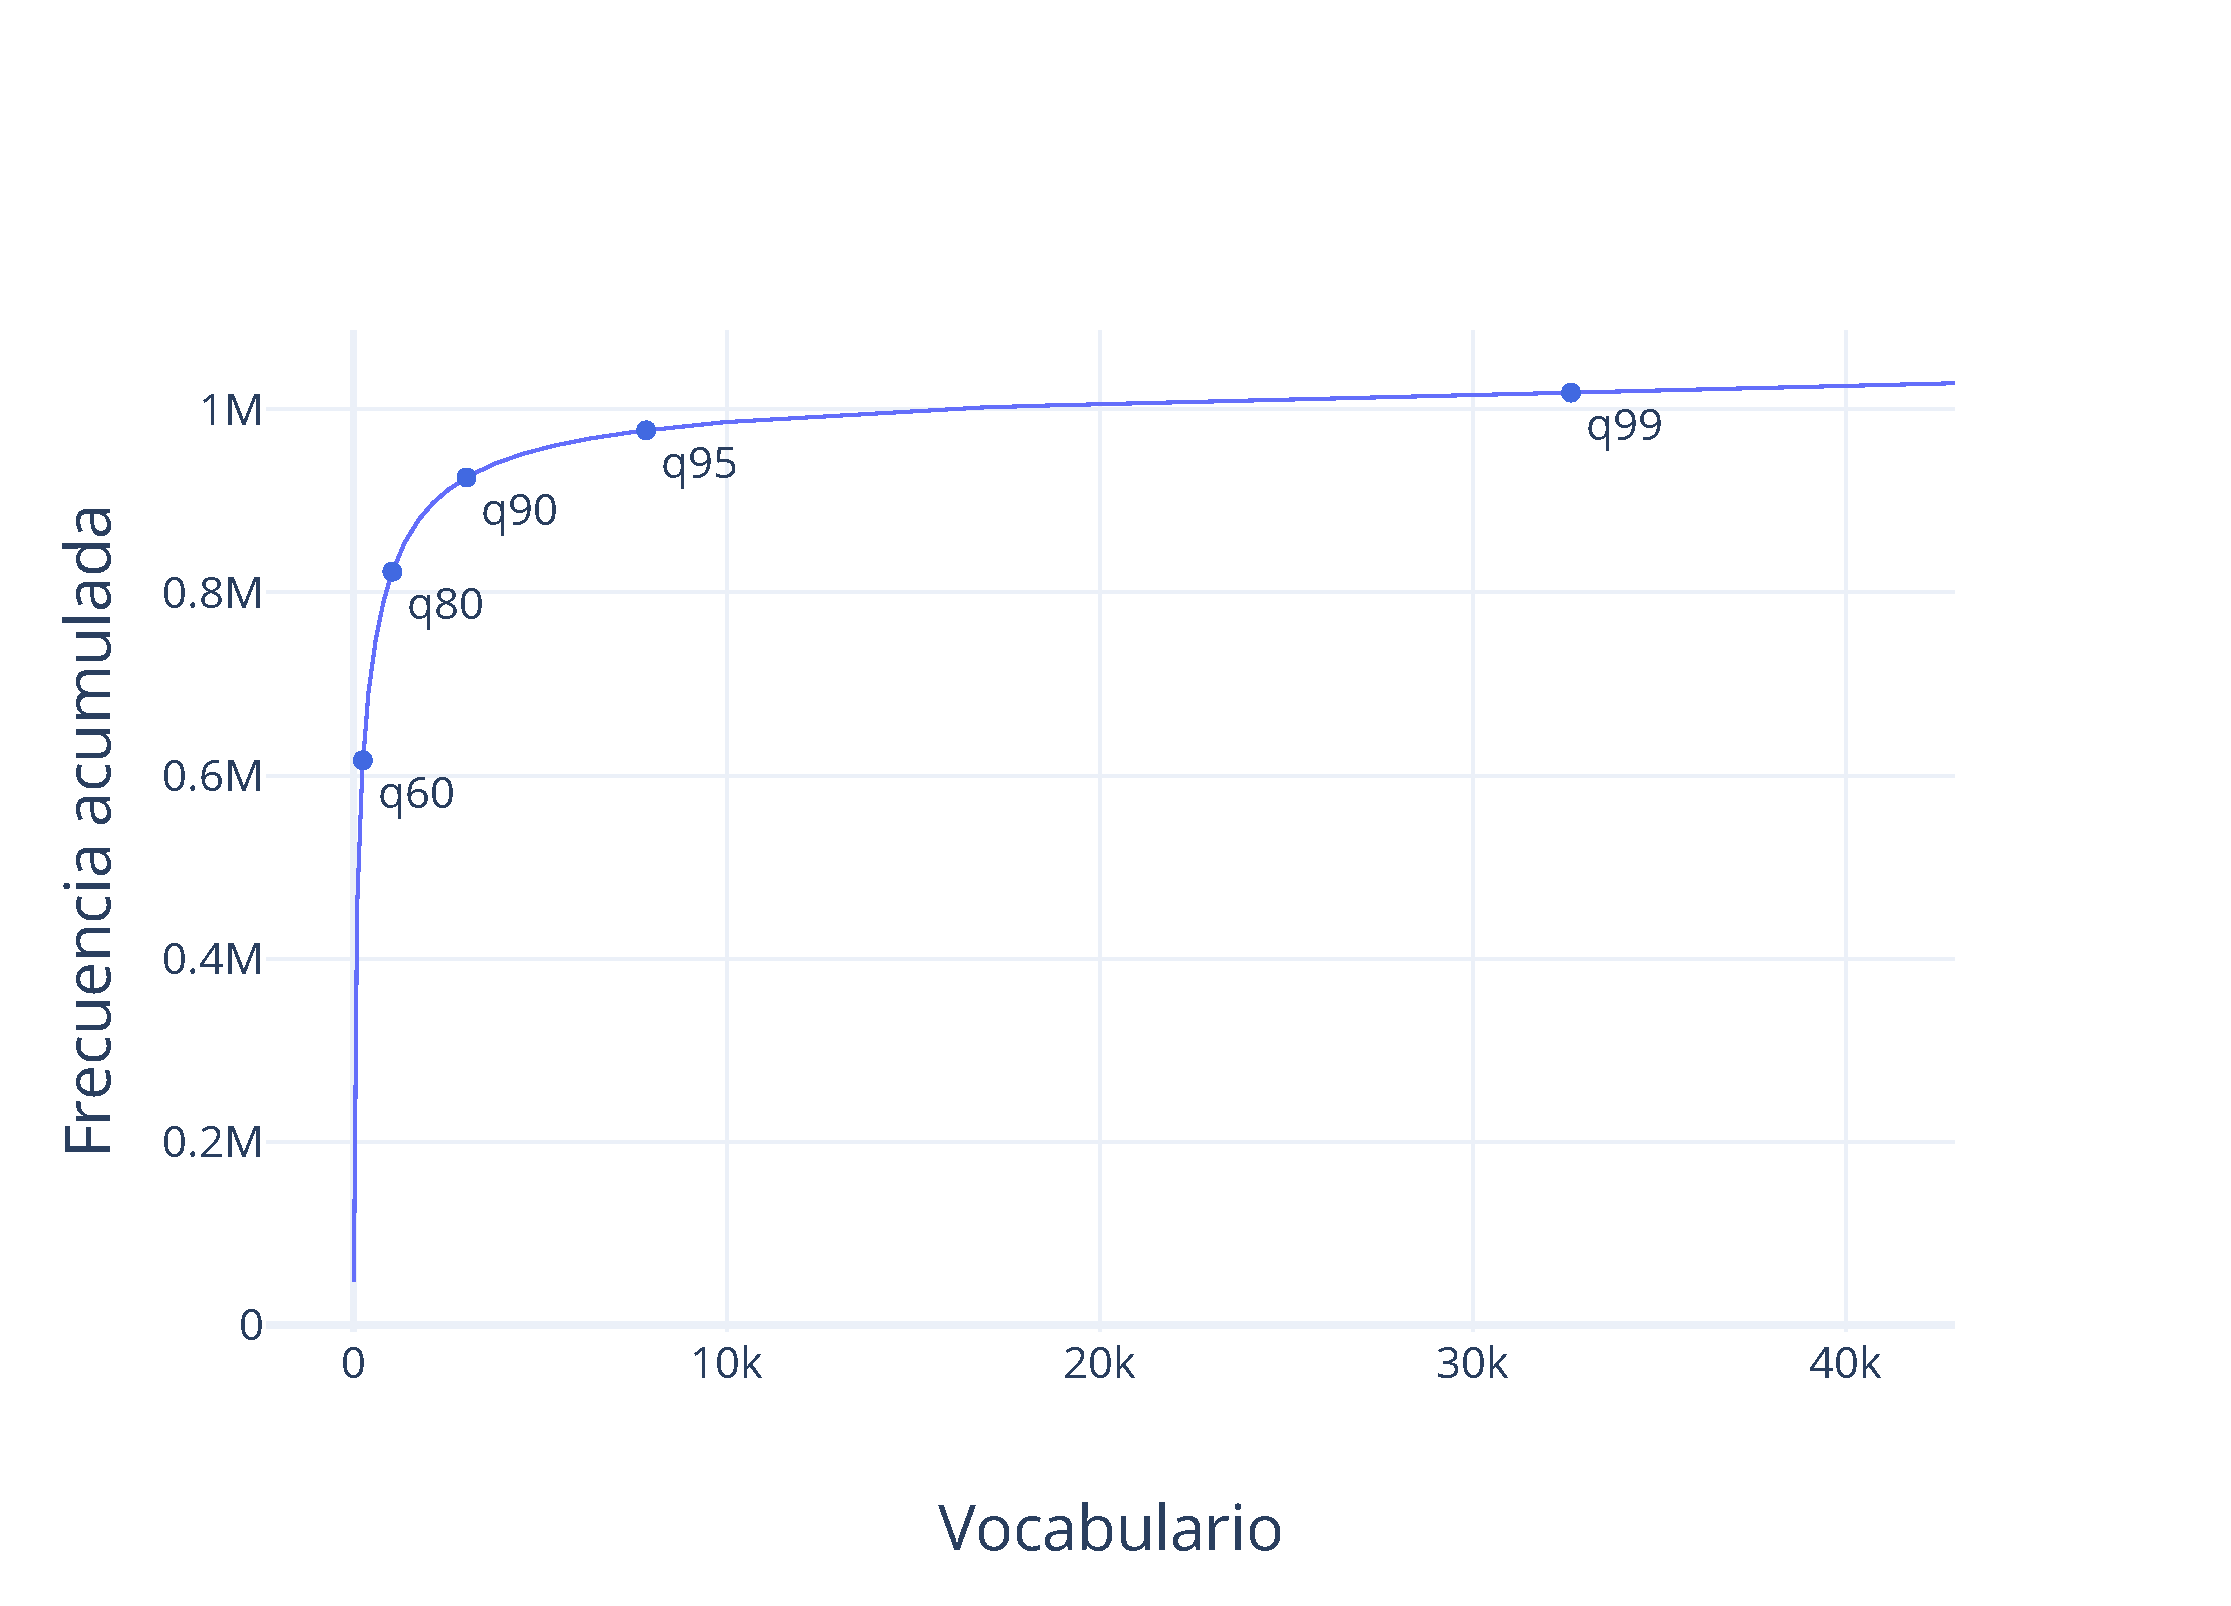
\includegraphics[width=0.8\textwidth]{ch4/cum_dist_2.eps}
    \caption{Frecuencia acumulada del vocabulario en orden decreciente de ocurrencia aplicando hasta el segundo nivel de procesamiento.}
    \label{img:cum_dist2}
\end{figure}

Hasta este nivel de procesamiento se tiene que al menos el 50\% de las palabras ocurren una única vez y al menos un 80\% tiene una frecuencia igual o menor a 4. El 95\% de la distribución acumulada puede ser explicada con 7837 palabras (un 18\% del vocabulario actual). En conclusión, la distribución de las palabras tiene una cola bastante pesada.\\

En la Figura \ref{img:cum_dist3} se muestra la nueva distribución tras eliminar las palabras que aparecen en menos del 0.1\% de los documentos de su época. En este nivel de procesamiento se redujo bastante el tamaño del vocabulario a 3148 (al rededor de 14 veces) sin alterar tan significativamente la cantidad de \textit{tokens} (alrededor de un 10\%), siendo ahora 925693 \textit{tokens}.\\

Luego se filtran palabras usando el vocabulario extraído del SUC. En la Figura \ref{img:cum_dist4} se observa que el vocabulario se redujo a 2902 y el la cantidad de \textit{tokens} a 901745. En este caso la variación no fue tan significativa, alrededor de un 8\% en el tamaño del vocabulario y de un 3\% en el caso de los \textit{tokens}.\\

A continuación, se eliminan las \textit{stopwords}, de la Figura \ref{img:cum_dist5} se puede observar que esto significó una reducción significativa de tanto el vocabulario como en el número de \textit{tokens}, respectivamente en 32\%(1960 palabras) y 45\%(495182 \textit{tokens}). La reducción abrupta en la cantidad de \textit{tokens} se debe principalmente a que las \textit{stopwords} son parte de las palabras más frecuentes dentro del corpus.\\

Por último, se eliminan los documentos con menos de 5 palabras, de la Figura \ref{img:cum_dist6} se puede observar que esto implicó una reducción de alrededor del 20\% en el tamaño del corpus y del 8\% en el número de \textit{tokens}.

\begin{figure}
    \centering
    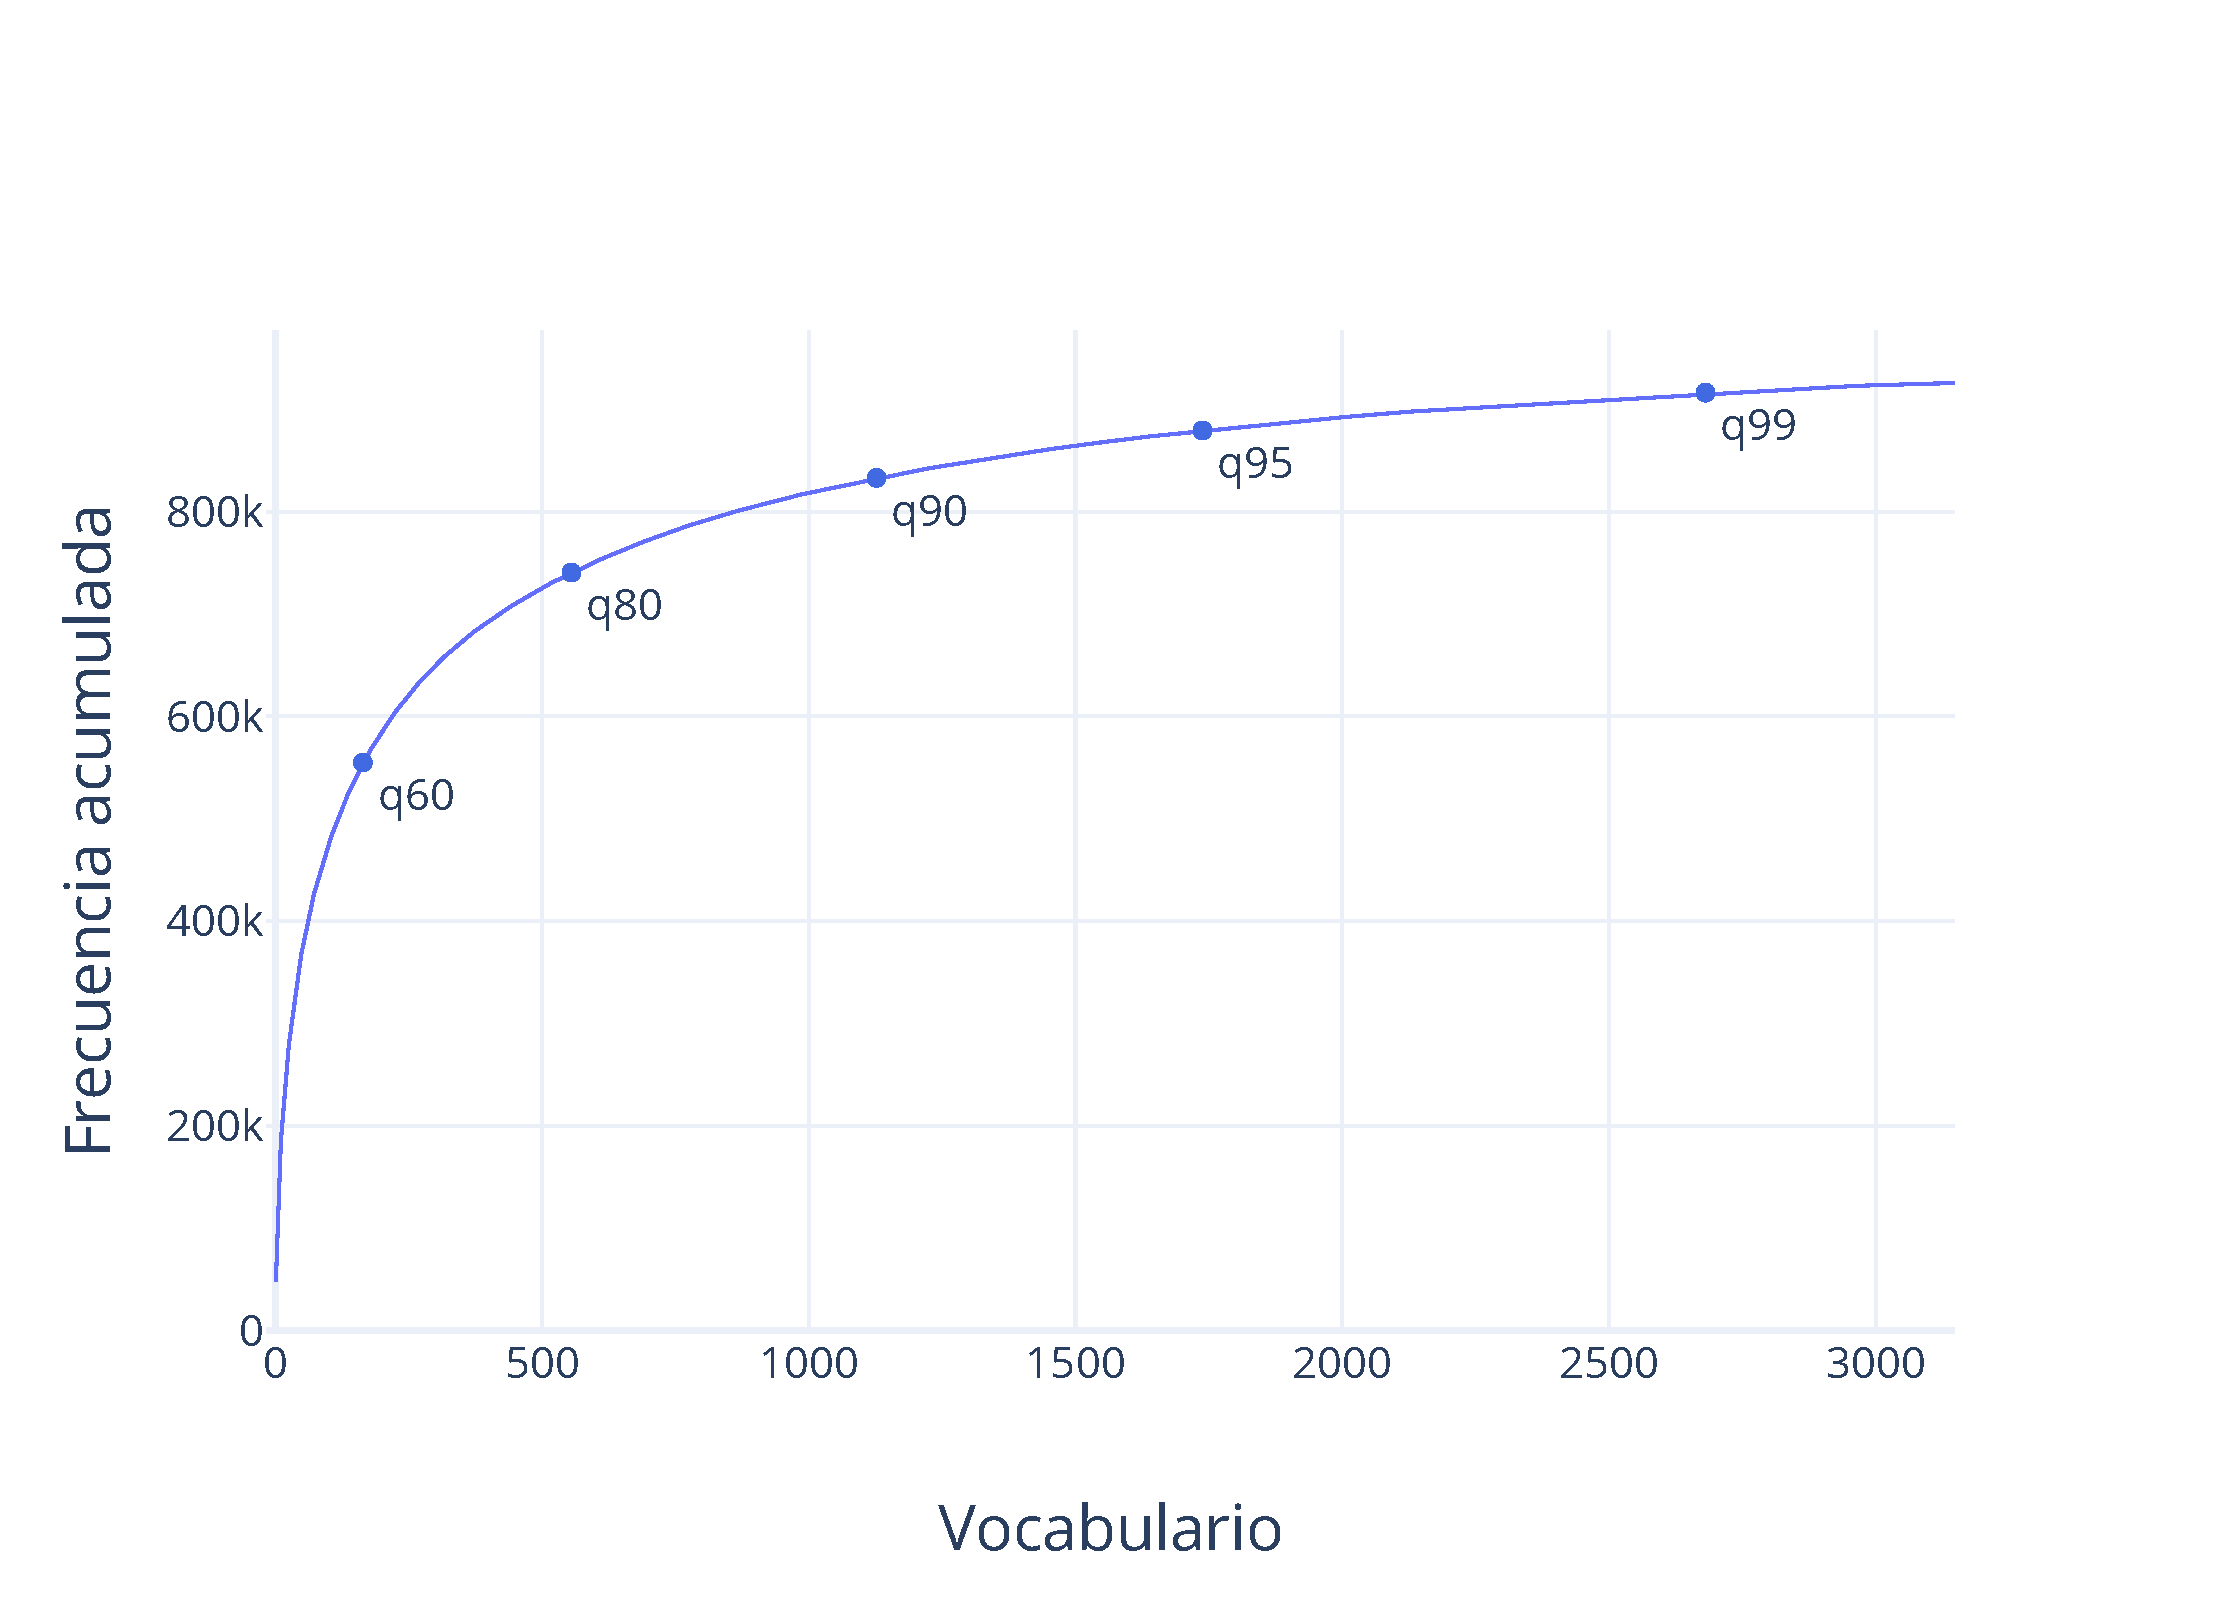
\includegraphics[width=0.8\textwidth]{ch4/cum_dist_3.eps}
    \caption{Frecuencia acumulada del vocabulario en orden decreciente de ocurrencia aplicando hasta el tercer nivel de procesamiento.}
    \label{img:cum_dist3}
\end{figure}

\begin{figure}
    \centering
    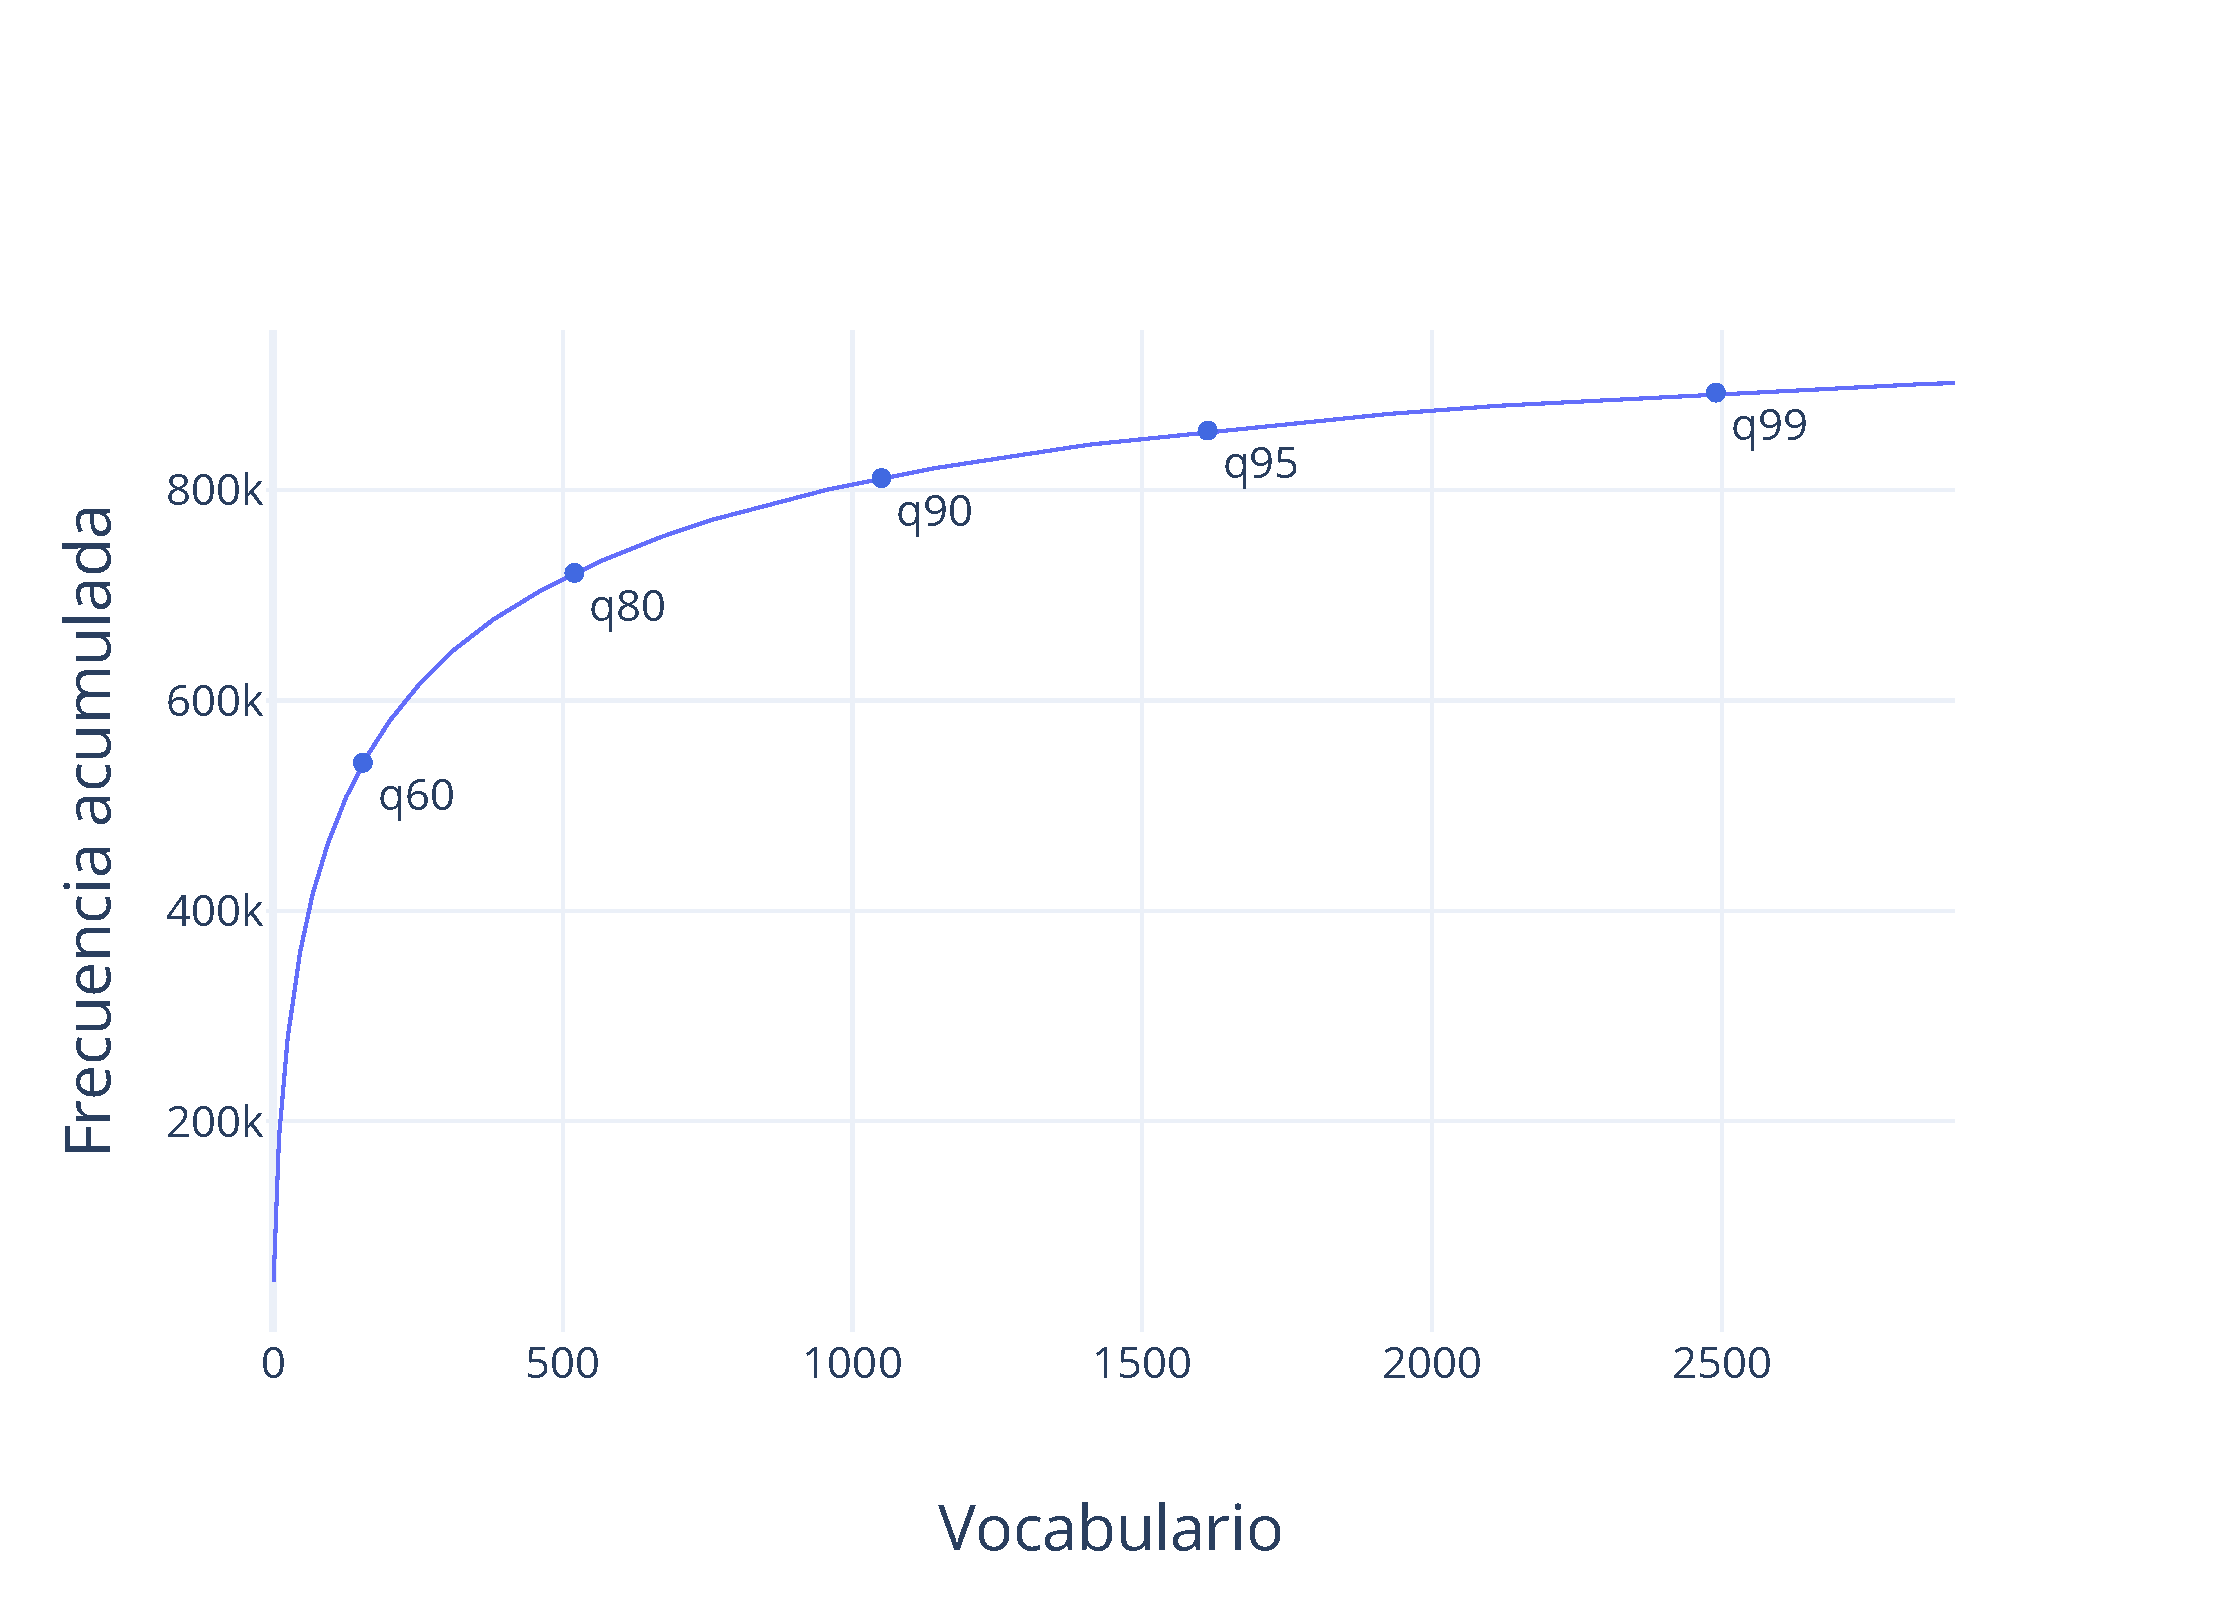
\includegraphics[width=0.8\textwidth]{ch4/cum_dist_4.eps}
    \caption{Frecuencia acumulada del vocabulario en orden decreciente de ocurrencia aplicando hasta el cuarto nivel de procesamiento.}
    \label{img:cum_dist4}
\end{figure}

\begin{figure}
    \centering
    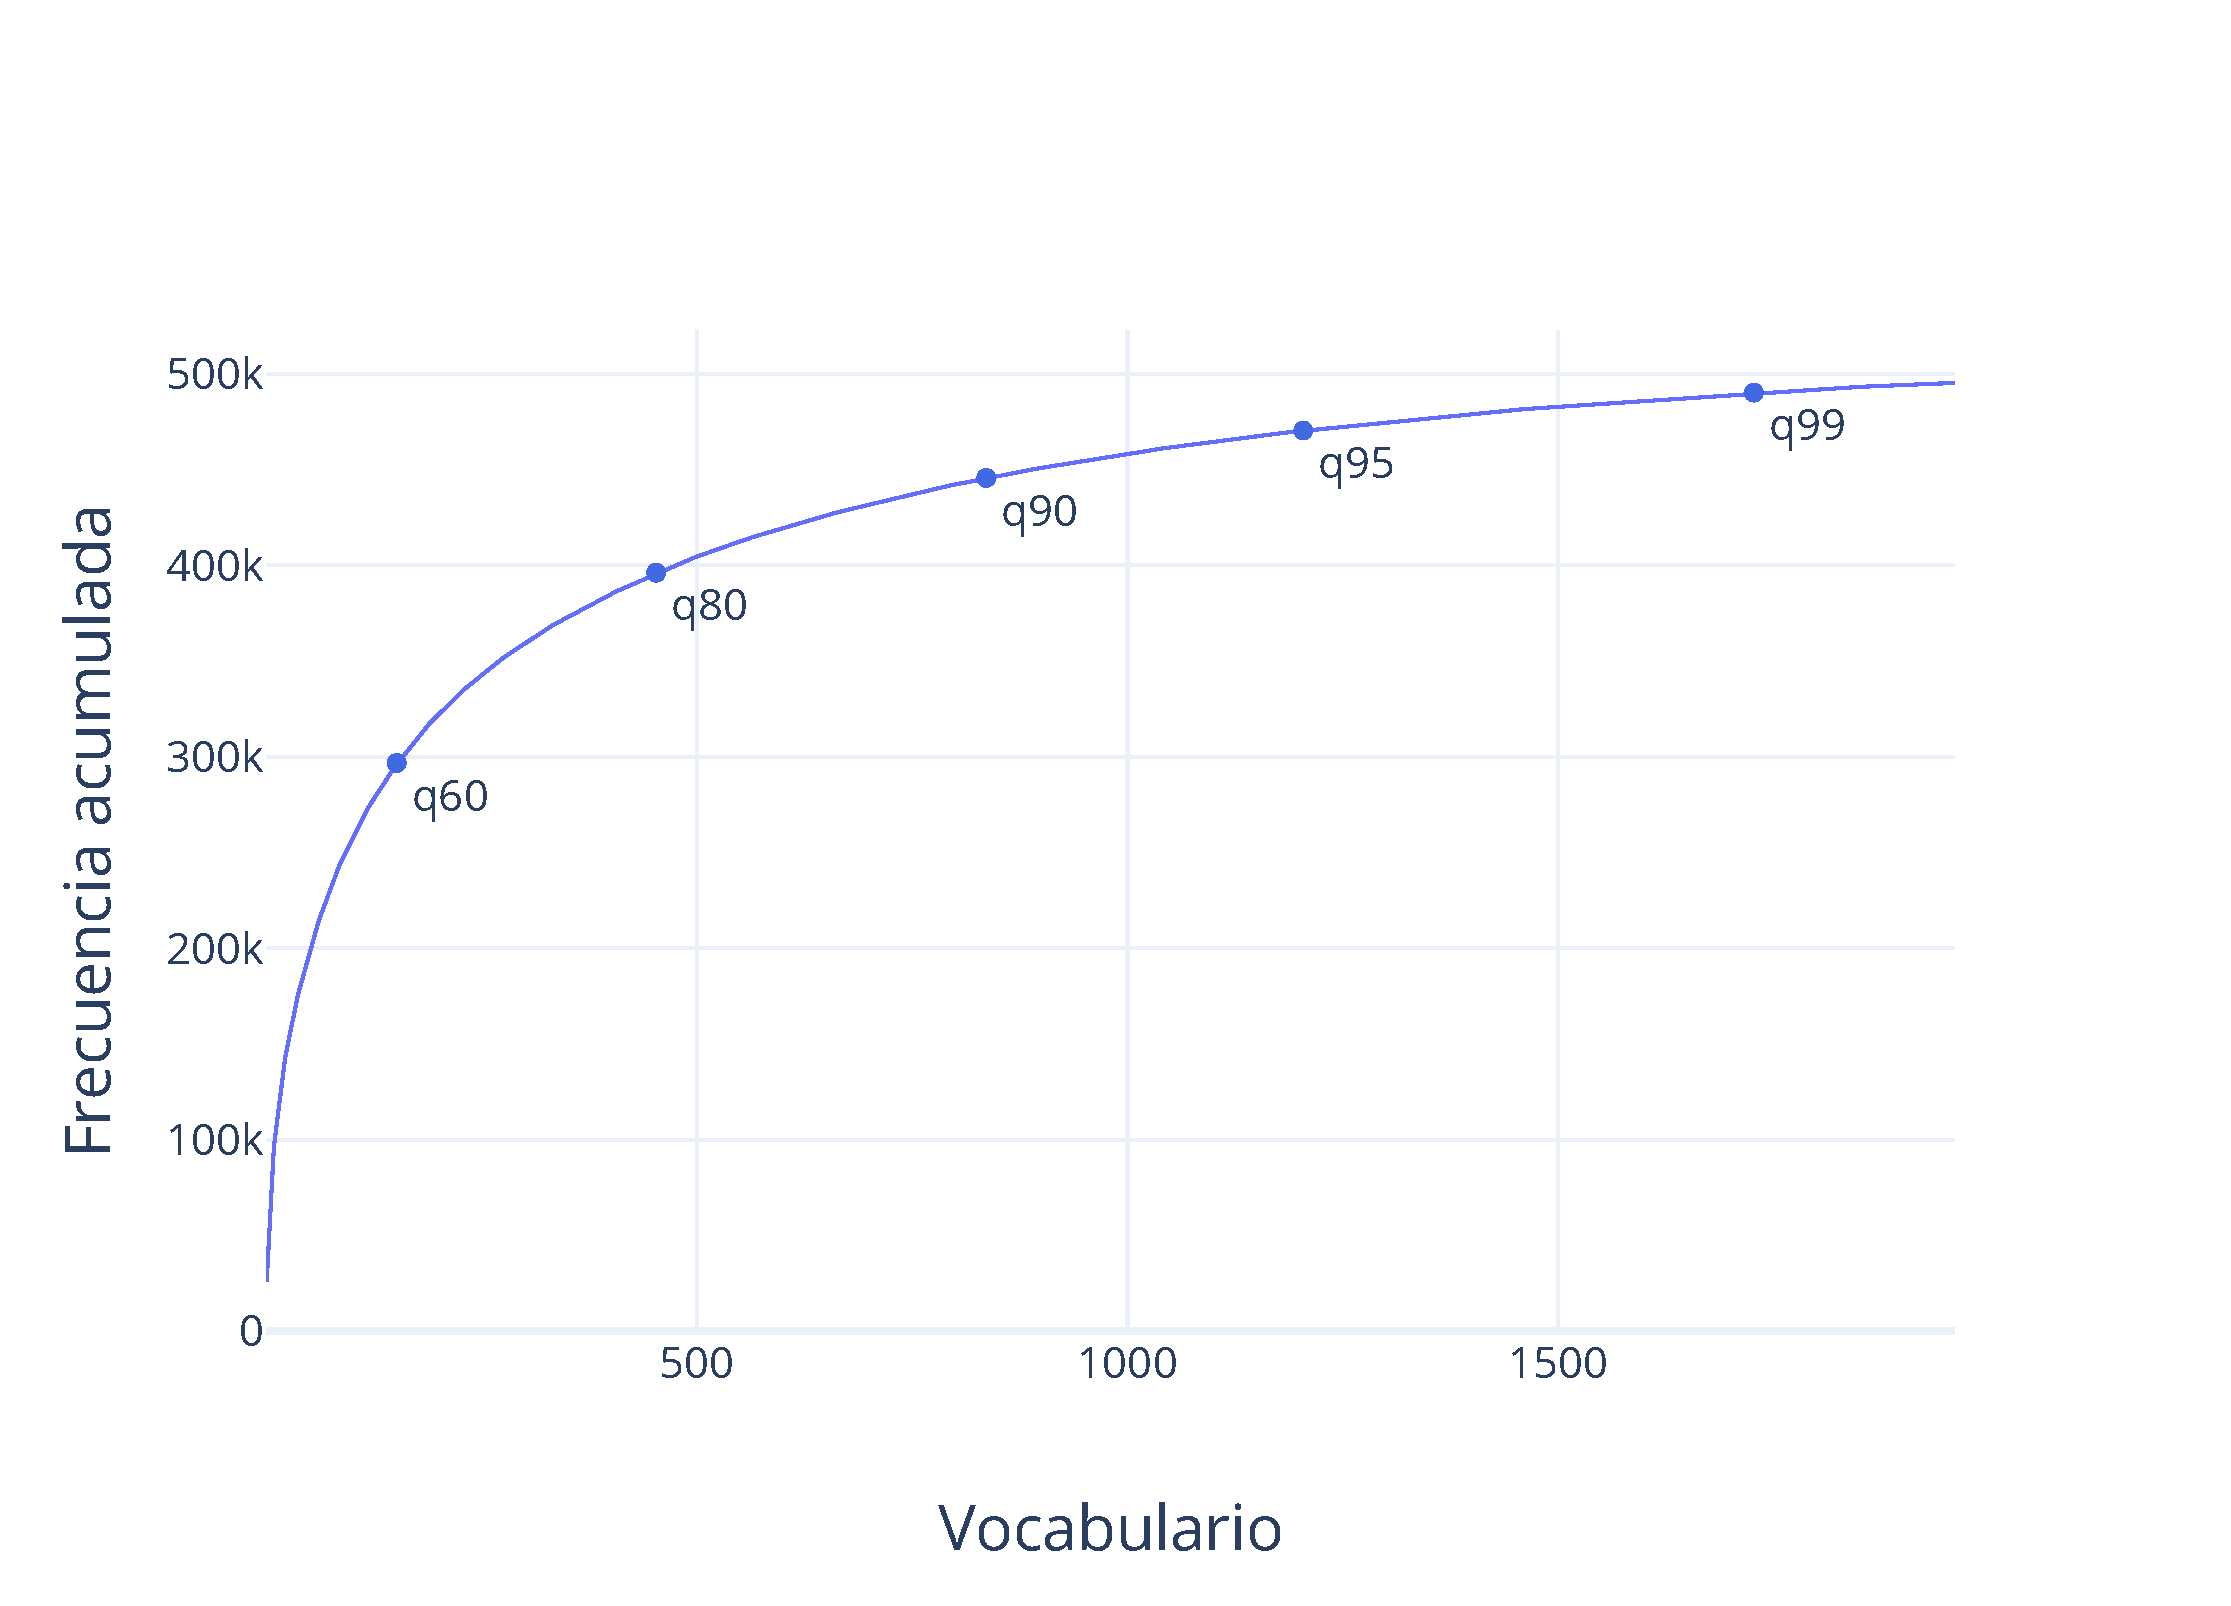
\includegraphics[width=0.8\textwidth]{ch4/cum_dist_5.eps}
    \caption{Frecuencia acumulada del vocabulario en orden decreciente de ocurrencia aplicando hasta el quinto nivel de procesamiento.}
    \label{img:cum_dist5}
\end{figure}

\begin{figure}
    \centering
    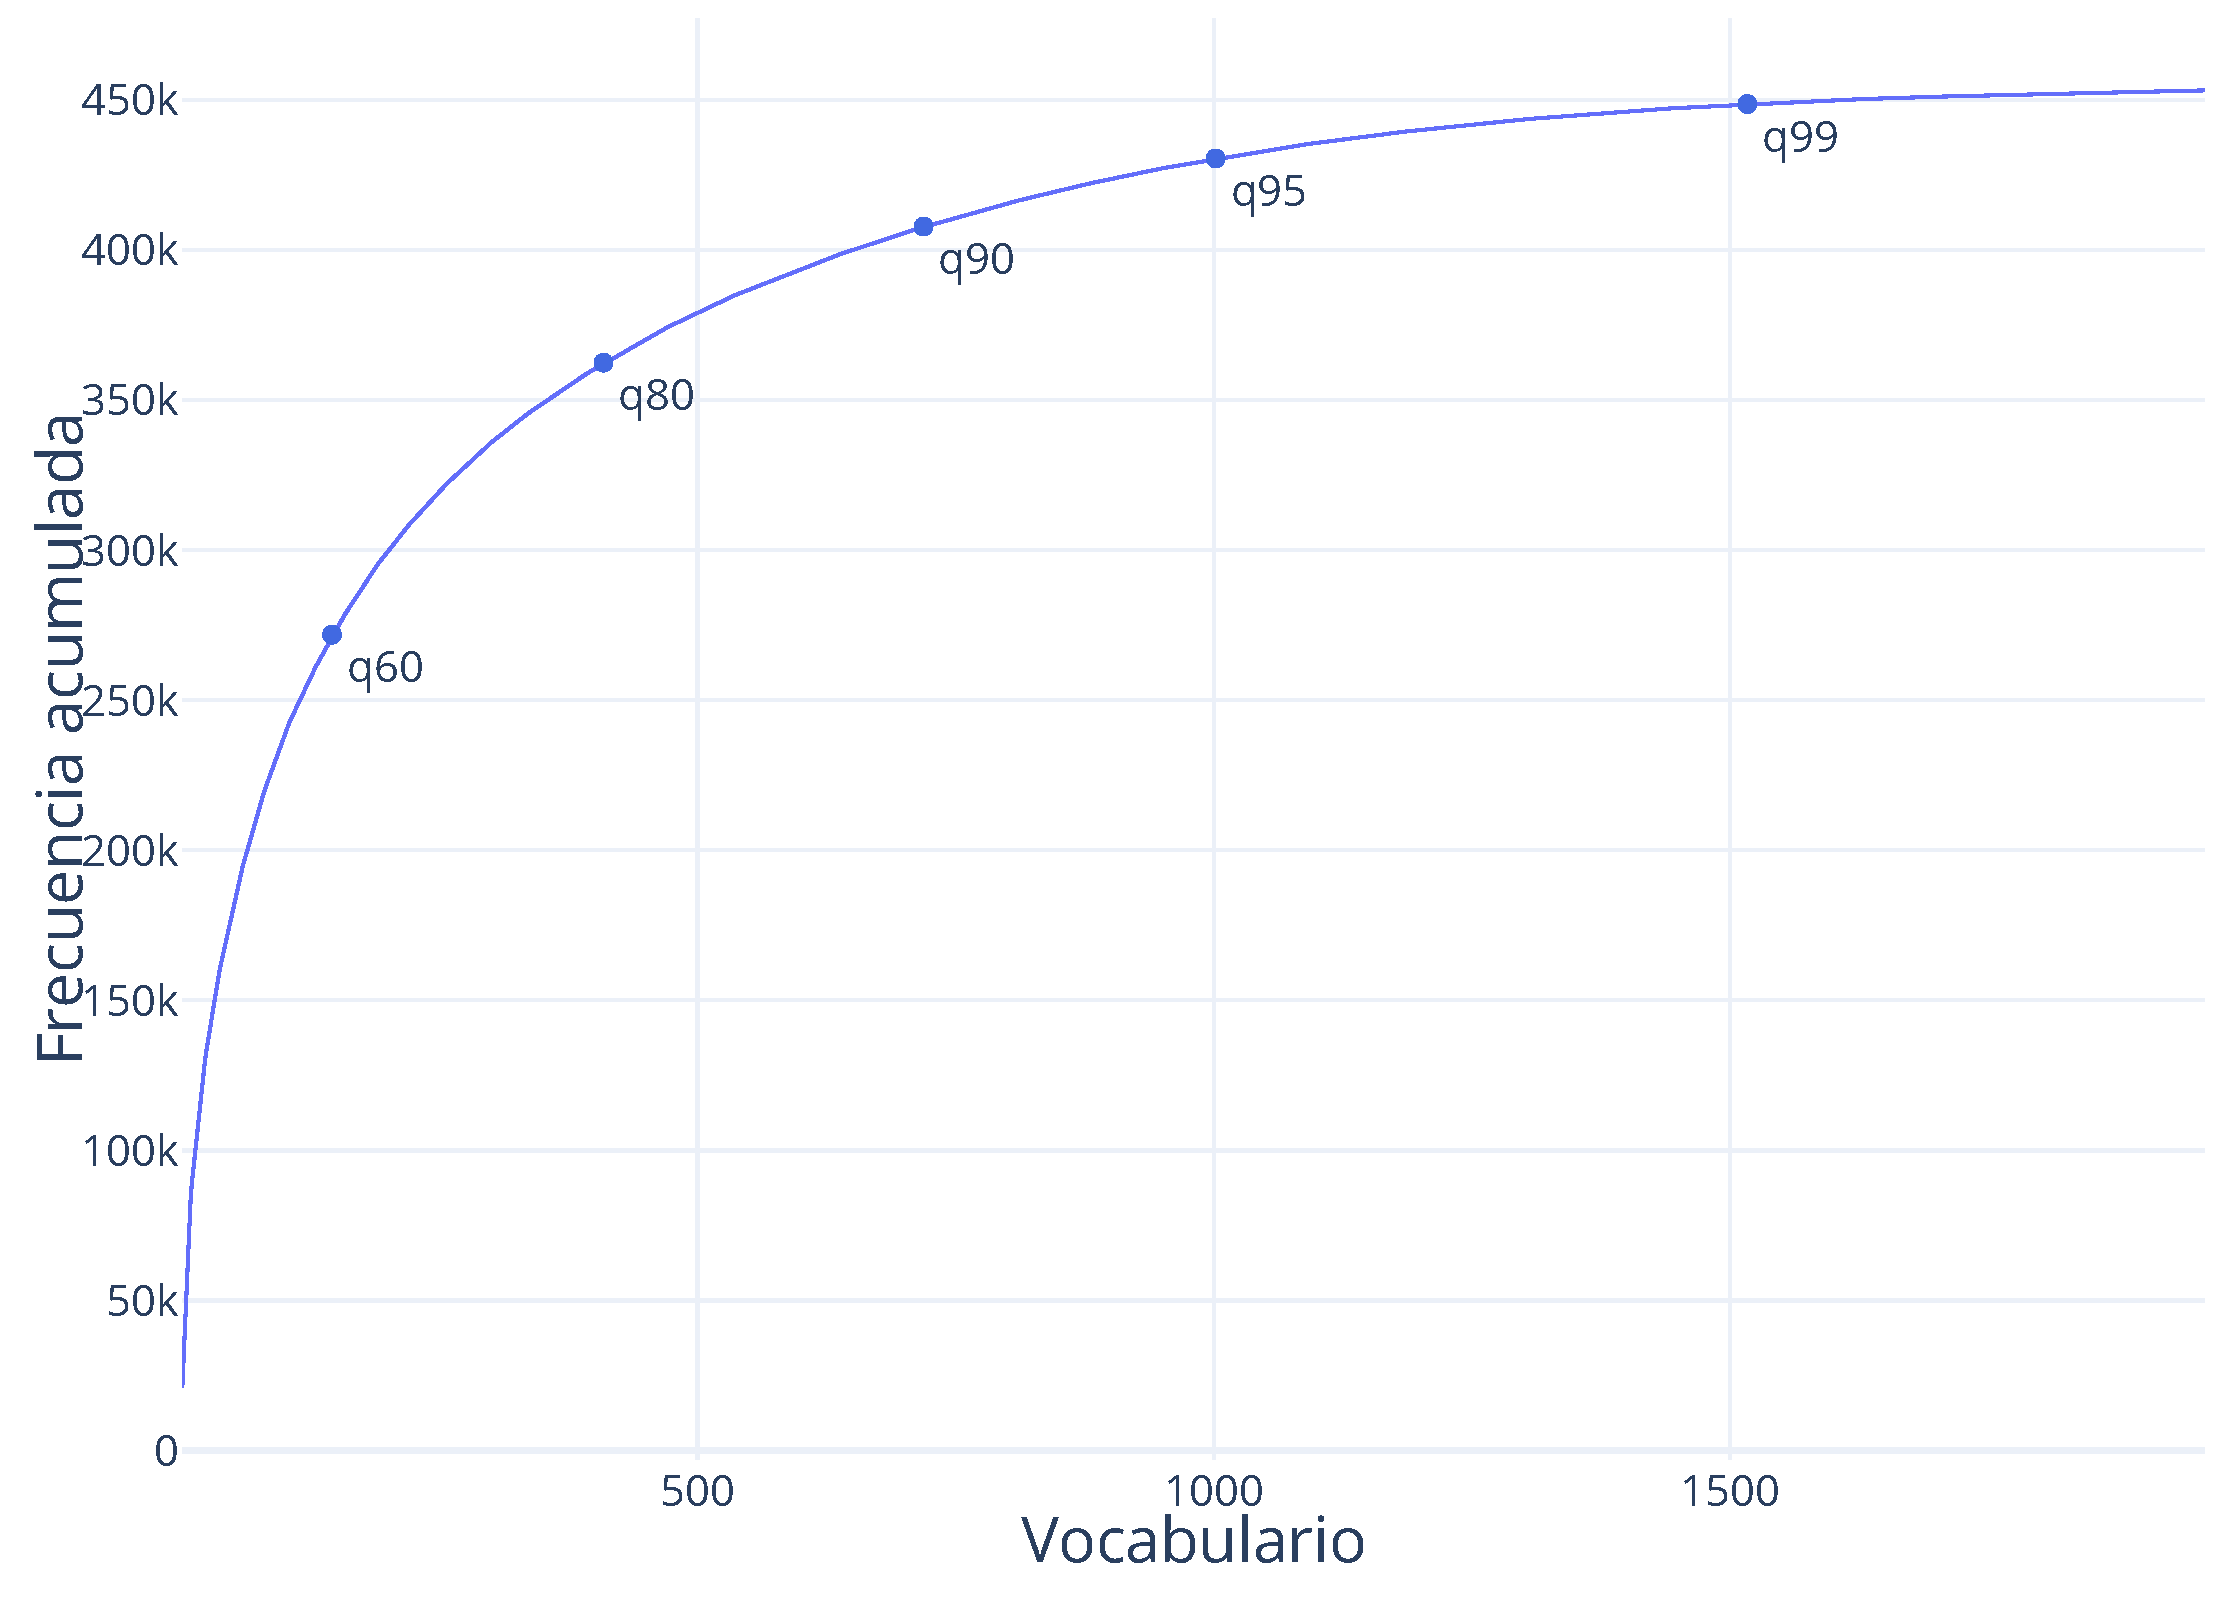
\includegraphics[width=0.8\textwidth]{ch4/cum_dist_6.eps}
    \caption{Frecuencia acumulada del vocabulario en orden decreciente de ocurrencia aplicando hasta el sexto nivel de procesamiento.}
    \label{img:cum_dist6}
\end{figure}

En la tabla \ref{table:processing_stats} se muestra un cuadro resumen con estadísticas del corpus bajo distintos niveles de procesamiento. De aquí se extrae que el tamaño del vocabulario, el corpus y la cantidad de \textit{tokens} se redujo en alrededor de un 98\%, un 20\% y un 76\% respectivamente.

\begin{table}[H]
    \begin{tabular}{|c|c|c|c|}
    \hline
    procesamiento & documentos & vocabulario & tokens  \\ \hline
    t             & 49015      & 93203       & 2030980 \\ \hline
    t+ch          & 49003      & 42921       & 1028412 \\ \hline
    t+ch+f        & 48988      & 3148        & 925693  \\ \hline
    t+ch+f+v      & 48988      & 2902        & 901745  \\ \hline
    t+ch+f+v+s    & 48566      & 1960        & 495182  \\ \hline
    t+ch+f+v+s+d  & 38850      & 1960        & 453206  \\ \hline
    \end{tabular}
    \caption{Estadísticas del corpus bajo distintos niveles de procesamientos, \textbf{t}: tokenización, \textbf{ch}: procesamiento de caracteres, \textbf{f}: filtro por frecuencia, \textbf{v}: filtro por vocabulario, \textbf{s}: eliminación de \textit{stopwords}, \textbf{d}: eliminación de documentos.}
    \label{table:processing_stats}
    \end{table}

En la tabla \ref{table:innovation_rate} se muestra el detalle del vocabulario para cada una de las épocas tras procesar el corpus, de aquí se extrae que en promedio un 12.83\% del vocabulario se olvida de una época a otra y un 18.92\% es nuevo, es otras palabras, en promedio alrededor de un 32\% del vocabulario no es común entre tópicos de épocas adyacentes. Esto justifica la necesidad por utilizar medidas de similitud robustas a cambios en el vocabulario, permitiendo así una comparación más justa entre tópicos que no tienen un vocabulario común.

\begin{table}[H]
    \begin{tabular}{|c|r|r|r|r|}
    \hline
    \textbf{época} & \multicolumn{1}{c|}{\textbf{t-1}} & \multicolumn{1}{c|}{\textbf{t}} & \multicolumn{1}{c|}{\textbf{t-1 {[}\%{]}}} & \multicolumn{1}{l|}{\textbf{t {[}\%{]}}} \\ \hline
    2              & 1145                              & 1187                            & 14.41                                      & 18.08                                    \\ \hline
    3              & 1187                              & 1281                            & 13.56                                      & 21.48                                    \\ \hline
    4              & 1281                              & 1329                            & 13.35                                      & 17.10                                    \\ \hline
    5              & 1329                              & 1405                            & 12.57                                      & 18.28                                    \\ \hline
    6              & 1405                              & 1537                            & 10.25                                      & 19.64                                    \\ \hline
    \end{tabular}
    \caption{Evolución del vocabulario en el tiempo, \textbf{t-1}: corresponde al vocabulario del período anterior a la época respectivame,\textbf{t-1}: corresponde al vocabulario de la época actual, \textbf{t-1[\%]}
    : porcentaje de palabras del período $t-1$ que ya no están en el período $t$ y \textbf{t[\%]}: porcentaje de palabras del período $t$ que no están en el período $t-1$.}
    \label{table:innovation_rate}.
\end{table}



\section{Análisis cuantitativo de resultados}
\label{sec:quantative}
\todoredo[inline]{Rehacer}

% Al aplicar HDP de forma independiente en cada una de los épocas se obtuvo el siguiente número de tópicos [8, 10, 9, 8, 8, 9].

% \subsubsection{Distribución acumulada de los tópicos}
% En la figura \ref{img:cum_dist3} se muestra la distribución acumulada promedio de los tópicos, se tiene que en promedio un 8.54\% y 21.42\% del vocabulario se puede capturar un 80\% y 95\% respectivamente de la distribución acumulada de los tópicos, además, para un 99\% de los tópicos basta con un 37\% del vocabulario para capturar el 95\% de su distribución acumulada, por tanto, una representación incompleta de los tópicos usando las palabras más probables que capturan el 80\% de la distribución acumulada trae consigo una disminución importante en el tamaño del vocabulario\todoredo{Rehacer}. 

% \begin{figure}
%     \centering
%     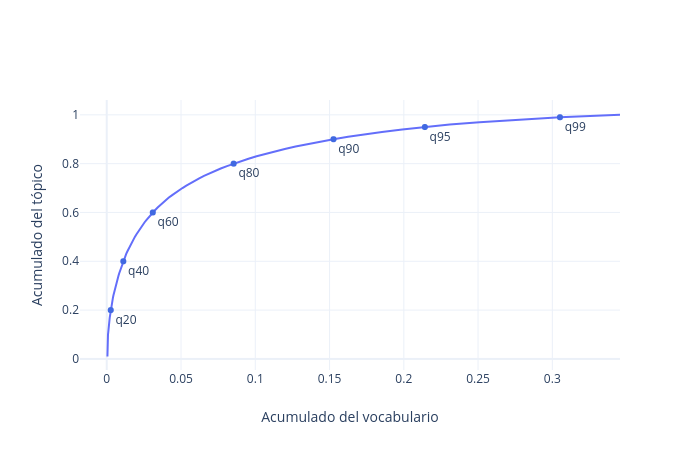
\includegraphics[width=0.8\textwidth]{ch3/cum_dist_3.png}
%     \caption{Distribución acumulada promedio de los tópicos en función del vocabulario. El punto (x,y) en el gráfico corresponde a la fracción x del vocabulario que explica la fracción y de la distribución acumulada del tópico. Los puntos corresponden a los cuantiles 60\%, 80\%, 90\%, 95\% y 99\%.}
%     \label{img:cum_dist3}
% \end{figure}\todoredo{Rehacer}

% \subsubsection{Construcción del grafo temporal}

% El modelo propuesto considera tres hiperparámetros:
% \begin{itemize}
%     \item $q \in [0,1]$: para el cálculo de WMD se utilizan las palabras más probables del tópico que explican un 100q\% de la distribución acumulada del tópico. Este parámetro genera un nuevo tópico (se normaliza para sumar 1) con un vocabulario más reducido.
%     \item $\lambda \in [0,1]$: este parámetro pondera la probabilidad de la palabra dentro del tópico con su exclusividad. El nuevo tópico generado es normalizado para sumar 1.
%     \item $\zeta \in [0,1]$: punto operante de la cdf del grafo inicial, permite definir el cuantil que se usará como úmbral para eliminar arcos con similitud menor a este. 
% \end{itemize}\todo{Marco teórico}

% Para entender de mejor manera la influencia de cada uno de estos parámetros se hizó un etiquetado de los arcos del grafo temporal, asignando un 1 a los arcos que deberían estar presente y 0 a los que no. Luego, se hizó una búsqueda a través de la siguiente grilla de parámetros, $\lambda \in \{0.2, 0.4, 0.6, 0.8, 1.0\}$, $q \in \{0.2, 0.4, 0.6, 0.8, 0.9, 0.95\}$ y $\zeta \in \{0.05, 0.10, ..., 0.90, 0.95\}$. \todo{Marco teórico y diseño de experimento}\\

% Como métrica de evaluación se propone \textit{F-score}, definida por:
% \begin{align}
%     F-score = 2\times \frac{\text{precision}\cdot \text{recall}}{\text{precision}+\text{recall}}
% \end{align}
% \todoredo{Usar métrica acorde al marco teórico}
% , donde \textit{recall} es la tasas de acierto sobre la clase positiva (presencia de un arco) y \textit{precision} es la tasa de acierto de las predicciones sobre la clase positiva. Esta métrica permite balancear la acertividad con la precisión, así una configuración que no pode ningún arco tendra un \textit{recall}=1, pero un bajo \textit{precision} (notar que el númerador decrece más rápido que el denominador). \\

% De la figura \ref{img:f_score} se observa que \textit{F-score} tiende a ser creciente en función de $\zeta$, esto se debe a que menor $\zeta$ más falsos positivos (pues son más arcos los que sobreviven) empeorando así el \textit{precision} y por consecuencia el \textit{F-score}. Las configuraciones óptimas ocurren en su mayoría en $\zeta=0.95$ con excepción de tres configuraciones de las treinta posibles de $q\times \lambda$, las cuales se dan en $\zeta=0.9$ para los parámetros $q=0.2$ con $\lambda \in \{0.8, 1\}$ y $q=0.4$ con $\lambda=0.2$, sin embargo, el valor óptimo alcanzado es bastante cercano al obtenido con $\zeta=0.95$. En cuanto a $\lambda$ se observa que no existen muchas diferencias entre $\lambda\in\{0.6, 0.8, 1.0\}$ a diferencia de $\lambda \in \{0.2, 0.4\}$ que suele estar significativamente por debajo de las otras curvas, además se observa una dominancia débil en $\lambda$, es decir, en el $\zeta$ óptimo dado un $(q, \lambda)$ un $\lambda$ mayor no es peor. En el caso del parámetro $q$ se observa que para $q\geq 0.6$ el óptimo obtenido para $\lambda\geq 0.4$ es el mismo, en cambio para $q=0.4$ esto se cumple para todo $\lambda\geq 0.6$ y con $q=0.2$ para $\lambda \geq 0.8$.\todoredo{Rehacer} 

% \begin{figure}
%     \centering
%     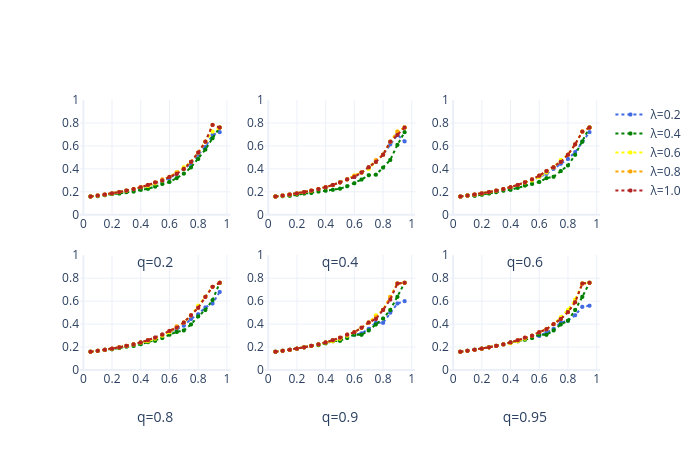
\includegraphics[width=1\textwidth]{ch3/f_score.png}
%     \caption{F-score (eje vertical) para diferentes configuraciones de los hiperparámetros $q$, $\zeta$ (eje horizontal) y $\lambda$.}
%     \label{img:f_score}
% \end{figure}\todoredo{Rehacer}

% De la tabla \ref{table:f_score} se observa que la configuración óptima se alcanza con $q=0.2$ con $\zeta=0.9$, además esto ocurre tanto para $\lambda=0.8$ como $\lambda=1.0$, por lo que es escoje la configuración $(q, \zeta, \lambda) = (0.2, 0.9, 1.0)$ para construir el grafo temporal. En la figura \ref{img:cdf} se observa la distribución acumulada de la similitud para el grafo completamente conectado, por lo que el para $zeta=0.9$ el úmbral viene siendo 0.21.\todoredo{Rehacer}

% \begin{table}[H]
%     \begin{tabular}{|c|c|c|c|c|}
%     \hline
%     \textbf{q} & \textbf{zeta} & \textbf{recall} & \textbf{precision} & \textbf{f-score} \\ \hline
%     0.2        & 0.9           & 0.87            & 0.71               & 0.78             \\ \hline
%     0.4        & 0.95          & 0.61            & 1                  & 0.76             \\ \hline
%     0.6        & 0.95          & 0.61            & 1                  & 0.76             \\ \hline
%     0.8        & 0.95          & 0.61            & 1                  & 0.76             \\ \hline
%     0.9        & 0.95          & 0.61            & 1                  & 0.76             \\ \hline
%     0.95       & 0.95          & 0.61            & 1                  & 0.76             \\ \hline
%     \end{tabular}
%     \caption{Configuración de $\zeta$ para cada $q$ que máximiza el \textit{F-score}.}
%     \label{table:f_score}
% \end{table}\todoredo{Rehacer}

% \begin{figure}
%     \centering
%     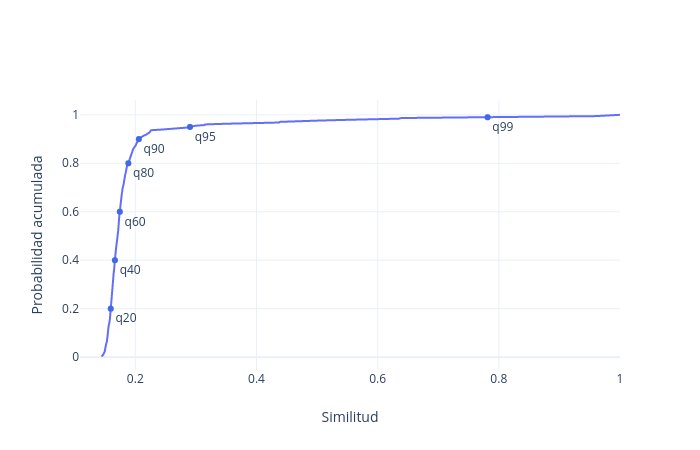
\includegraphics[width=0.8\textwidth]{ch3/cdf.png}
%     \caption{Estimación empírica de la función de distribución acumulada (cdf) de la similitud entre tópicos correspondiente al grafo temporal completamente conectado para la configuración óptima $(q, \lambda)=(0.2, 1.0)$.}
%     \label{img:cdf}
% \end{figure}\todoredo{Rehacer}

% En la figura \ref{img:speedup} se observa que la configuración óptima es en promedio 184 veces más eficiente que $q=0.95$, esto se debe a que $q=0.2$ es un 0.3\% del vocabulario (6 palabras en promedio) y $q=0.95$ alrededor de un 21\% (488 palabras en promedio).\todoredo{Rehacer}


% \begin{figure}
%     \centering
%     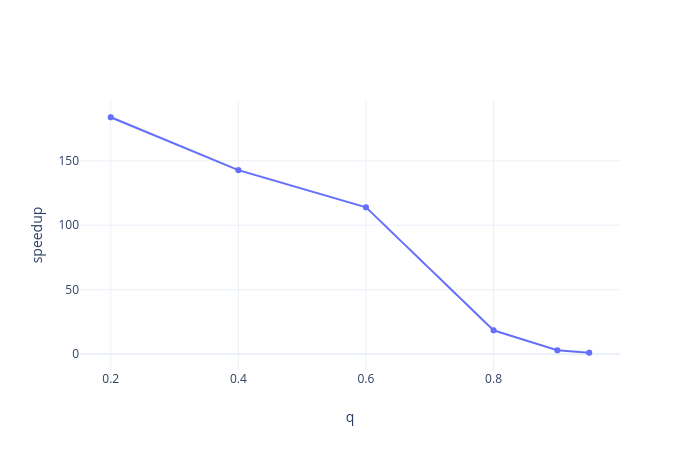
\includegraphics[width=1\textwidth]{ch3/speedup.png}
%     \caption{Speedup promedio de la construcción del grafo en función de $q$. El speedup 1 equivale al tiempo más lento el cual está asciado a $q=0.95$ que es el valor de $q$ más grande y por ende con menor reducción de vocabulario de los tópicos a la hora de computar WMD.}
%     \label{img:speedup}
% \end{figure}\todoredo{Rehacer}

% %\ref{img:ground_truth} y \ref{img:pruned_graph}
% %conteo de arcos y blabla
% %asociacion a tamaño de los topicos 
% %no hablar todavía del significado de los tópicos

% \begin{figure}
%     \centering
%     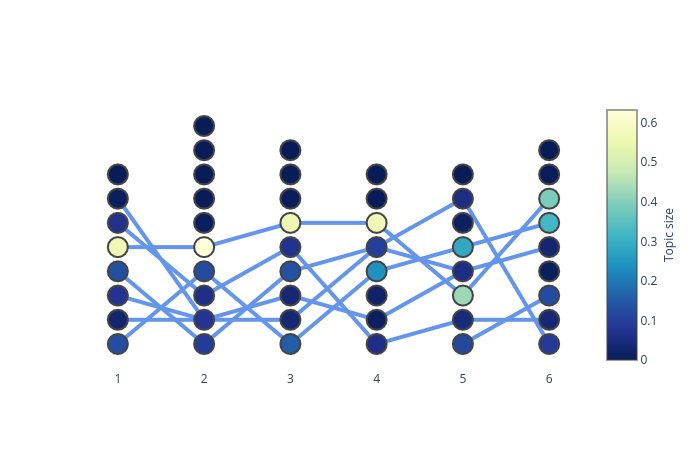
\includegraphics[width=0.8\textwidth]{ch3/ground_truth.png}
%     \caption{Grafo temporal etiquetado.}
%     \label{img:ground_truth}
% \end{figure}\todoredo{Rehacer}

% \begin{figure}
%     \centering
%     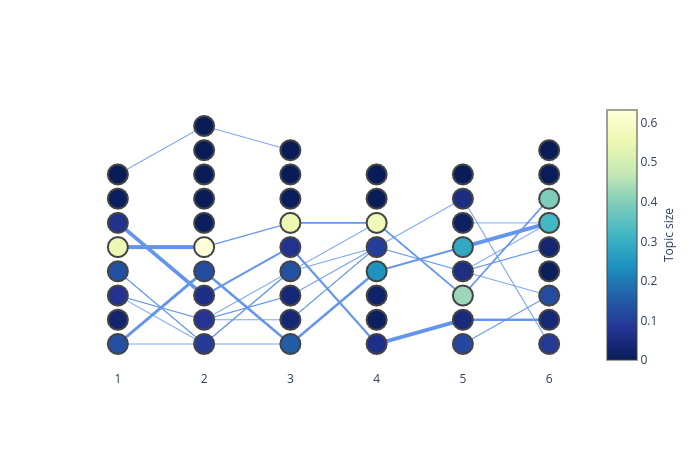
\includegraphics[width=0.8\textwidth]{ch3/pruned_graph.png}
%     \caption{Grafo temporal obtenido a partir de la configuración óptima de parámetros $(q, \lambda, \zeta) = (0.2, 1.0, 0.9)$.}
%     \label{img:pruned_graph}
% \end{figure}\todoredo{Rehacer}

\section{Análisis cualitativo de resultados}
\label{sec:qualitative}
\todosec[inline]{Análisis cualitativo de tópicos}